% Toolbar icon: estimateError — a posteriori error estimation. A coarse
% straight chord under the smooth curve it approximates, with the gap between
% them hatched: that gap IS the quantity the estimator measures (recovered
% minus raw). Distinct from `quality` (element-shape bands) because this is
% about the SOLUTION's error, not the mesh's geometry.
\documentclass[tikz,border=2mm]{standalone}
\usetikzlibrary{arrows.meta,calc,shapes.geometric}
\begin{document}
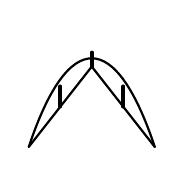
\begin{tikzpicture}[line width=1.3pt, line cap=round, line join=round, x=1mm,y=1mm]
  % The exact solution: a smooth arc.
  \draw[thick] (-8,-6) .. controls (-3,9) and (3,9) .. (8,-6);
  % The discrete approximation: two straight segments through the same ends.
  \draw[thick] (-8,-6) -- (0,4.2) -- (8,-6);
  % The error between them, as vertical ticks.
  \draw (-4,-0.9) -- (-4,1.7);
  \draw (0,4.2) -- (0,6.0);
  \draw (4,-0.9) -- (4,1.7);
\end{tikzpicture}
\end{document}
